
\documentclass[12pt, a4paper]{article}
\usepackage[utf8]{inputenc}
\usepackage[spanish]{babel}
\usepackage{graphicx} 
\usepackage{geometry}
\usepackage{hyperref}
\usepackage{float}
\usepackage{titlesec}
\usepackage{booktabs}
\usepackage{caption}
\usepackage{amsmath} % <--- AGREGADO: Para corregir el error de \text

% Configuración de márgenes
\geometry{top=2.5cm, bottom=2.5cm, left=3cm, right=3cm}

% Información del documento
\title{Primer Avance del Proyecto: Sistema de Gestión de Citas Médicas con Análisis Predictivo}
\author{Brian Steven Beltrán Reina \\ Edwin Geovanni Guerra Cruz \\ Edgar Alessandro López Martinez}
\date{\today}

\begin{document}
	
	% -----------------------------------------------------------------------------------
	% PORTADA
	% -----------------------------------------------------------------------------------
	\begin{titlepage}
		\centering
		% Asegúrate de subir un archivo llamado logo.png
		
\includegraphics[width=0.3\textwidth]{Logo.png} \par\vspace{1cm}
		
		{\scshape\LARGE Universidad Católica de El Salvador \par}
		\vspace{0.5cm}
		{\scshape\Large Facultad de Ingeniería y Arquitectura \par}
		\vspace{0.5cm}
		{\scshape\Large Ingeniería en Desarrollo de Software \par}
		\vspace{1.5cm}
		
		{\huge\bfseries Sistema de Gestión de Citas Médicas para Clínica \par}
		\vspace{0.5cm}
		{\large Primer Avance (20\%) \par}
		\vspace{1.5cm}
		
		\textbf{Cátedra:} \\
		Programación de Base de Datos \par
		\vspace{0.5cm}
		
		\textbf{Catedrático:} \\
		Ing. José Ernesto Erazo Linares \par
		\vspace{1cm}
		
		\textbf{Integrantes:} \\
		Brian Steven Beltrán Reina \\
		Edwin Geovanni Guerra Cruz \\
		Edgar Alessandro López Martinez \par
		\vspace{2cm}
		
		{\large \today \par}
	\end{titlepage}
	
	% -----------------------------------------------------------------------------------
	% ÍNDICE
	% -----------------------------------------------------------------------------------
	\tableofcontents
	\newpage
	
	% -----------------------------------------------------------------------------------
	% 1. ALCANCE DEL PROYECTO
	% -----------------------------------------------------------------------------------
	\section{Alcance del Proyecto a Realizar}
	
	El proyecto consiste en el desarrollo de una plataforma web integral para la gestión clínica, diseñada para optimizar el flujo de trabajo operativo y potenciar la toma de decisiones mediante inteligencia artificial.
	
	\subsection{Funcionalidades Principales}
	El sistema abarcará los siguientes módulos funcionales:
	\begin{itemize}
		\item \textbf{Gestión de Usuarios y Roles:} Administración de perfiles para doctores, pacientes y personal administrativo.
		\item \textbf{Gestión de Citas Médicas:} Programación, reprogramación y cancelación de citas, permitiendo visualizar la disponibilidad de los doctores en tiempo real.
		\item \textbf{Expediente Clínico Electrónico:} Registro de consultas, signos vitales (peso, talla, presión arterial), diagnósticos (CIE-10) y recetas médicas.
		\item \textbf{Farmacia e Inventario:} Control de stock de medicamentos, alertas de stock mínimo y vinculación directa con las recetas emitidas.
		\item \textbf{Módulo de Inteligencia Artificial (Analytics):} Integración con un microservicio en Python para analizar datos históricos y generar predicciones sobre ausentismo de pacientes y riesgos de salud basados en signos vitales.
	\end{itemize}
	
	\subsection{Problemática que Resuelve}
	Actualmente, muchas clínicas enfrentan problemas como la pérdida de expedientes físicos, la ineficiencia en la gestión de inventarios y una alta tasa de ausentismo en las citas ("No-Show"). 
	
	Nuestra base de datos y sistema resuelven esto centralizando la información, garantizando la integridad de los datos médicos y proporcionando herramientas predictivas que permiten a la clínica tomar medidas preventivas (ej. recordatorios personalizados) para reducir pérdidas económicas y mejorar la atención al paciente.
	
	% -----------------------------------------------------------------------------------
	% 2. VIABILIDAD DEL PROYECTO
	% -----------------------------------------------------------------------------------
	\section{Viabilidad del Proyecto}
	
	\subsection{Viabilidad Técnica}
	El proyecto es altamente viable tecnológicamente debido al uso de un stack moderno y robusto:
	\begin{itemize}
		\item \textbf{Backend:} Java con Spring Boot, estándar en la industria para sistemas empresariales seguros y escalables.
		\item \textbf{Base de Datos:} PostgreSQL, un motor relacional potente capaz de manejar transacciones complejas y grandes volúmenes de datos.
		\item \textbf{Machine Learning:} Python (Pandas, Scikit-learn), líder indiscutible en ciencia de datos.
		\item \textbf{Infraestructura:} Uso de Docker para la contenerización, asegurando que el despliegue sea consistente en cualquier entorno.
	\end{itemize}
	
	\subsection{Impacto en el Entorno Informático}
	\textbf{Positivo:} La adopción de una arquitectura de microservicios (separando la lógica de negocio en Java y el análisis en Python) fomenta la mantenibilidad y escalabilidad. Además, el uso de estándares abiertos reduce la dependencia de licencias costosas.
	
	\textbf{Negativo/Riesgos:} La curva de aprendizaje para integrar dos stacks diferentes (Java y Python) y la gestión de la infraestructura en contenedores requiere un nivel técnico avanzado, lo cual se mitiga con una buena documentación y prácticas DevOps.
	
	% -----------------------------------------------------------------------------------
	% 3. DIAGRAMAS DE ARQUITECTURA DE SOFTWARE
	% -----------------------------------------------------------------------------------
	\section{Diagramas de Arquitectura de Software}
	
	En esta sección se detallan los diagramas que modelan el comportamiento y la estructura del sistema.
	
	\subsection{Diagrama de Casos de Uso}
	Muestra las interacciones entre los actores (Paciente, Doctor, Admin) y el sistema.
	\begin{figure}[H]
		\centering
		 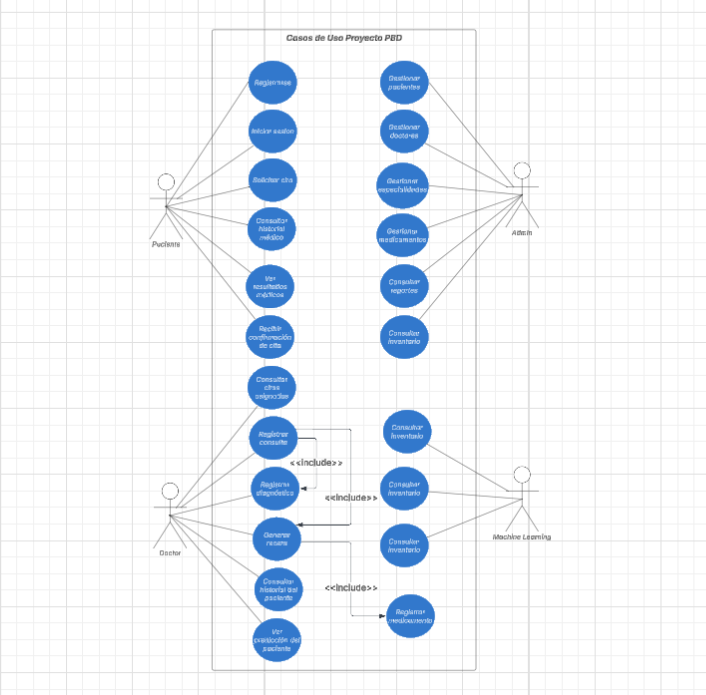
\includegraphics[width=0.8\textwidth]{casos.png} 
		\caption{Diagrama de Casos de Uso General}
	\end{figure}
	
	\subsection{Diagrama de Actividades}
	Flujo del proceso principal: Agendamiento y realización de una consulta médica.
	\begin{figure}[H]
		\centering
	 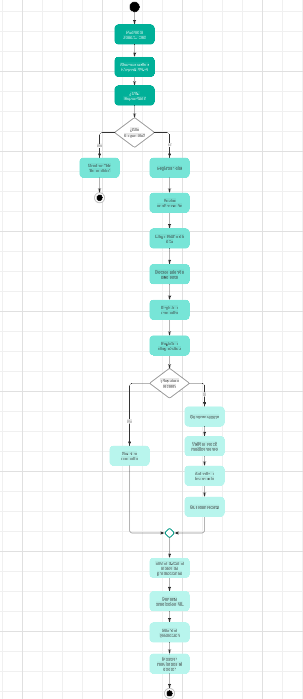
\includegraphics[width=0.8\textwidth]{actividades.png}
		\caption{Diagrama de Actividades: Proceso de Cita Médica}
	\end{figure}
	
	\subsection{Diagramas de Contexto (DFD)}
	
	\subsubsection{Diagrama de Contexto (Nivel 0)}
	\begin{figure}[H]
		\centering
		 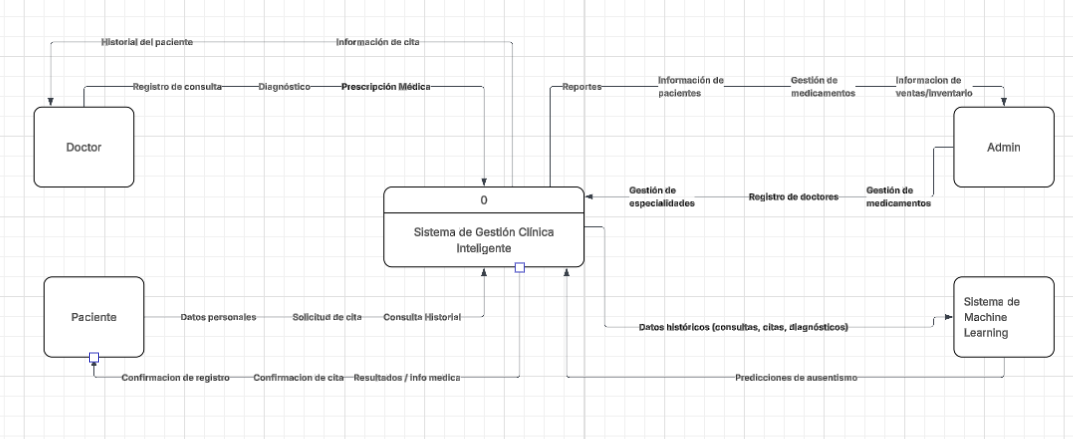
\includegraphics[width=0.8\textwidth]{0.png}
		\caption{Diagrama de Flujo de Datos - Nivel 0}
	\end{figure}
	
	\subsubsection{Diagrama de Nivel 1}
	\begin{figure}[H]
		\centering
		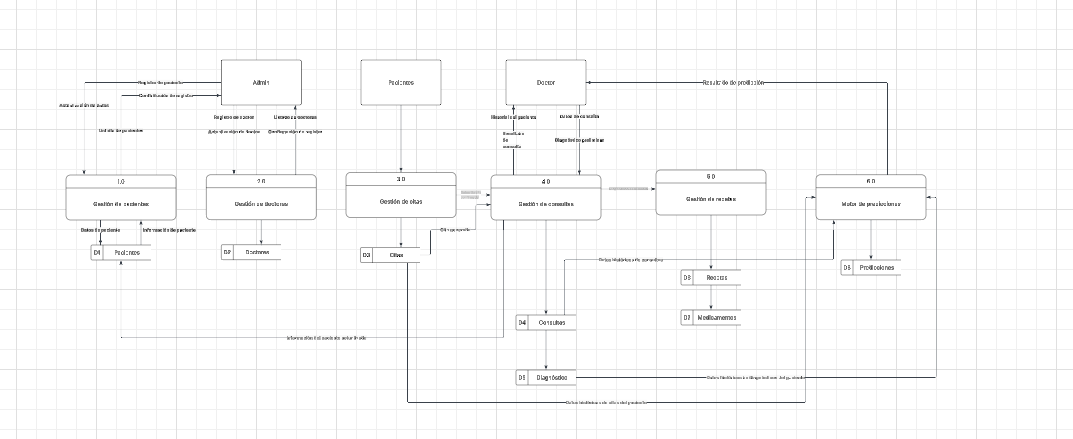
\includegraphics[width=0.8\textwidth]{1.png}
	
		\caption{Diagrama de Flujo de Datos - Nivel 1}
	\end{figure}
	
	\subsubsection{Diagrama de Nivel 2}
	\begin{figure}[H]
		\centering
		 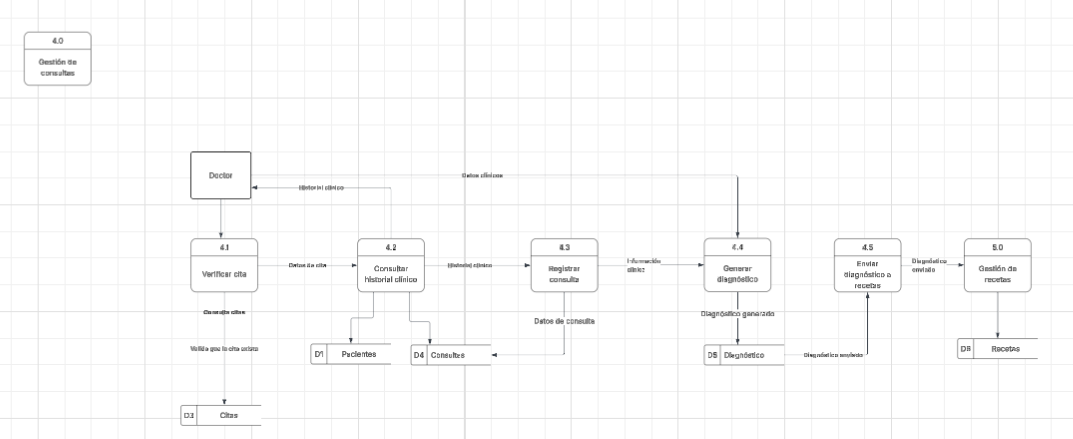
\includegraphics[width=0.8\textwidth]{2.png}
		\caption{Diagrama de Flujo de Datos - Nivel 2 (Proceso Específico)}
	\end{figure}
	
	\subsection{Arquitectura de la Aplicación}
	Arquitectura híbrida mostrando la comunicación entre Spring Boot, el contenedor de PostgreSQL y el servicio de Machine Learning en Python.
	\begin{figure}[H]
		\centering
		 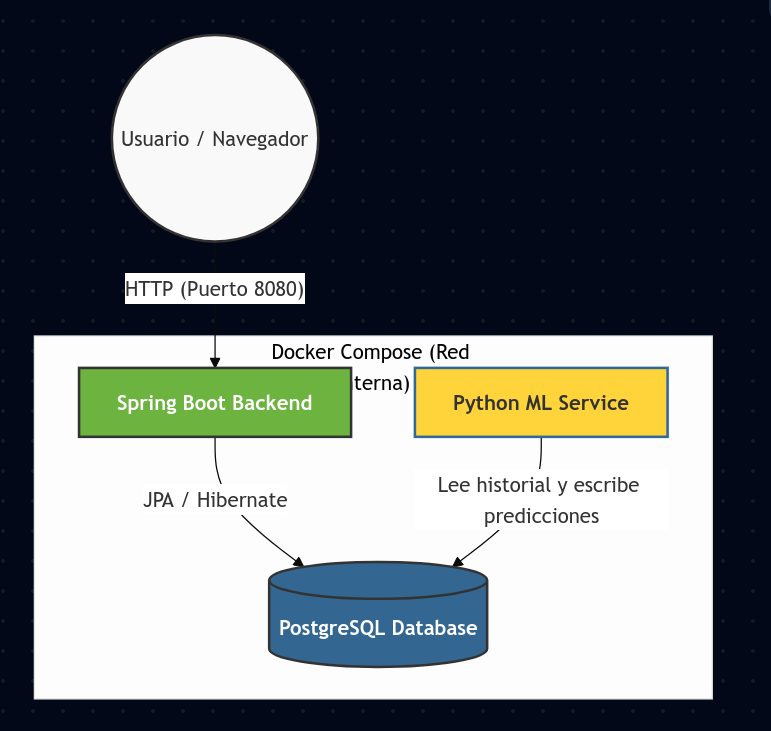
\includegraphics[width=0.8\textwidth]{arquitectura.png}
	
		\caption{Arquitectura de Microservicios y Contenedores}
	\end{figure}
	
	\subsection{Primer Diagrama Entidad-Relación (DER)}
	Modelo lógico de la base de datos PostgreSQL, incluyendo tablas clave como Pacientes, Doctores, Citas y Predicciones.
	\begin{figure}[H]
		\centering
		 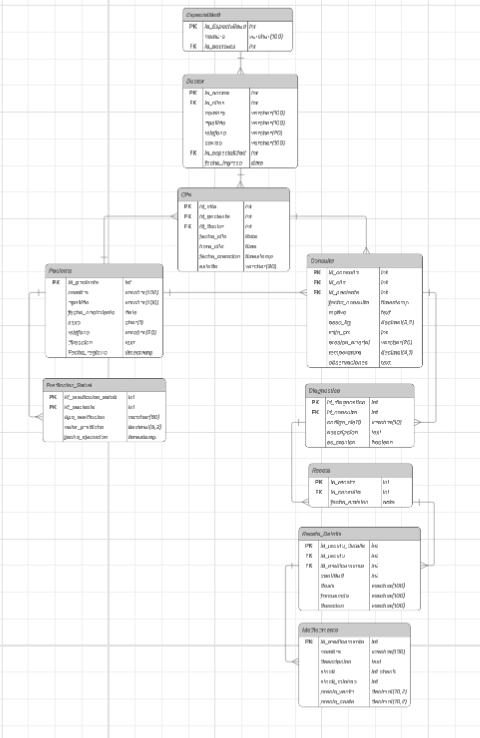
\includegraphics[width=0.9\textwidth]{der.png}
		\caption{Diagrama Entidad-Relación (Generado desde PostgreSQL)}
	\end{figure}
	
	% -----------------------------------------------------------------------------------
	% 4. ESTIMACIÓN Y COSTOS (COCOMO)
	% -----------------------------------------------------------------------------------
\section{Estimación y Costos (Método COCOMO)}

Para la estimación de costos y esfuerzo se ha utilizado el modelo \textbf{COCOMO Básico} en modo \textit{Orgánico}, ajustado al equipo de desarrollo conformado por 3 integrantes.

\textbf{Variables del modelo:}
\begin{itemize}
	\item \textbf{KLOC} (Miles de líneas de código estimadas): 4.5 KLOC
	\item \textbf{Equipo de Desarrollo:} 3 Personas (Brian Beltrán, Edwin Guerra, Edgar López)
	\item \textbf{Salario Mensual por Desarrollador:} \$800.00 USD (Promedio Junior)
	\item $a = 2.4$, $b = 1.05$ (Coeficientes para modo Orgánico)
\end{itemize}

\subsection{Cálculo de Esfuerzo (E)}
El esfuerzo representa la cantidad de trabajo requerido en meses/persona.
\[ E = a \times (KLOC)^b = 2.4 \times (4.5)^{1.05} \approx 11.64 \text{ Personas-Mes} \]

\subsection{Cálculo de Tiempo Real (T)}
Considerando que el equipo está compuesto por \textbf{3 integrantes} trabajando en paralelo, dividimos el esfuerzo total entre el número de desarrolladores:

\[ T_{real} = \frac{E}{\text{Nº Desarrolladores}} = \frac{11.64}{3} \approx 3.88 \text{ Meses} \]

\textit{Nota: Esto se alinea con la duración aproximada de un ciclo académico (4 meses).}

\subsection{Estimación de Costo Total del Proyecto}
El costo se calcula multiplicando el esfuerzo total por el salario mensual estimado.

\[ Costo = E \times \text{Salario} = 11.64 \times \$800.00 \]
\[ \textbf{Costo Total} = \textbf{\$9,312.00 USD} \]

\begin{table}[H]
	\centering
	\begin{tabular}{ll}
		\toprule
		\textbf{Concepto} & \textbf{Estimación} \\
		\midrule
		Líneas de Código (KLOC) & 4.5 \\
		Esfuerzo Total & 11.64 Personas-Mes \\
		Equipo de Trabajo & 3 Desarrolladores \\
		\textbf{Tiempo de Desarrollo} & \textbf{3.88 Meses} \\
		Salario Base (Mes) & \$800.00 \\
		\textbf{Costo Total del Software} & \textbf{\$9,312.00 USD} \\
		\bottomrule
	\end{tabular}
	\caption{Resumen de Estimación Económica (3 Integrantes)}
\end{table}
	
	% -----------------------------------------------------------------------------------
	% 5. METODOLOGÍAS ÁGILES
	% -----------------------------------------------------------------------------------
	\section{Metodologías Ágiles}
	
	El desarrollo se rige bajo el marco de trabajo \textbf{Scrum}, permitiendo entregas incrementales y adaptación a cambios.
	
	\subsection{Seguimiento del Desarrollo}
	\begin{itemize}
		\item \textbf{Sprints:} Ciclos de desarrollo de 2 semanas.
		\item \textbf{Herramientas:} Uso de Trello/Jira para el tablero Kanban (Backlog, En Progreso, Terminado) y GitHub para el control de versiones.
		\item \textbf{Daily Meetings:} Reuniones cortas de sincronización para identificar bloqueos.
	\end{itemize}
	
	\subsection{Planificación de Sprints Iniciales}
	\begin{itemize}
		\item \textbf{Sprint 0:} Configuración del entorno Docker, definición de la Base de Datos PostgreSQL y diseño de arquitectura.
		\item \textbf{Sprint 1:} Desarrollo del Backend (Spring Boot) para CRUD de Pacientes y Doctores.
		\item \textbf{Sprint 2:} Implementación del módulo de Citas y conexión con el servicio de ML en Python.
	\end{itemize}
	
	% -----------------------------------------------------------------------------------
	% 6. DOCUMENTACIÓN ADICIONAL E INNOVACIÓN
	% -----------------------------------------------------------------------------------
	\section{Documentación Adicional y Funcionalidades Innovadoras}
	
	\subsection{Funcionalidad Innovadora: Analítica Predictiva}
	A diferencia de los sistemas de gestión clínica tradicionales, nuestra base de datos incluye una estructura dedicada (\texttt{predicciones\_salud}) alimentada por algoritmos de Machine Learning.
	\begin{itemize}
		\item \textbf{Predicción de Ausentismo:} Analiza la fecha de creación de la cita vs. la fecha real para predecir la probabilidad de que un paciente no asista, permitiendo a la clínica confirmar con antelación.
		\item \textbf{Alertas de Salud:} Monitoreo de tendencias en signos vitales (presión arterial, peso) para sugerir intervenciones preventivas antes de un diagnóstico crítico.
	\end{itemize}
	
	\subsection{Documentación de API}
	Se utiliza **OpenAPI (Swagger)** para documentar automáticamente los endpoints REST generados por Spring Boot, facilitando la integración con el Frontend y aplicaciones móviles futuras.
	
	% -----------------------------------------------------------------------------------
	% 7. PROTOTIPOS DEL SISTEMA
	% -----------------------------------------------------------------------------------
	\section{Prototipos del Sistema}
	
	A continuación, se presentan los prototipos funcionales de las pantallas principales del sistema.
	
	\subsection{Pantalla de Inicio de Sesión}
	\begin{figure}[H]
		\centering
		 
\includegraphics[width=0.7\textwidth]{login.png}
	
		\caption{Prototipo de Acceso}
	\end{figure}
	
	\subsection{Dashboard Principal con Estadisticas}
	\begin{figure}[H]
		\centering
		 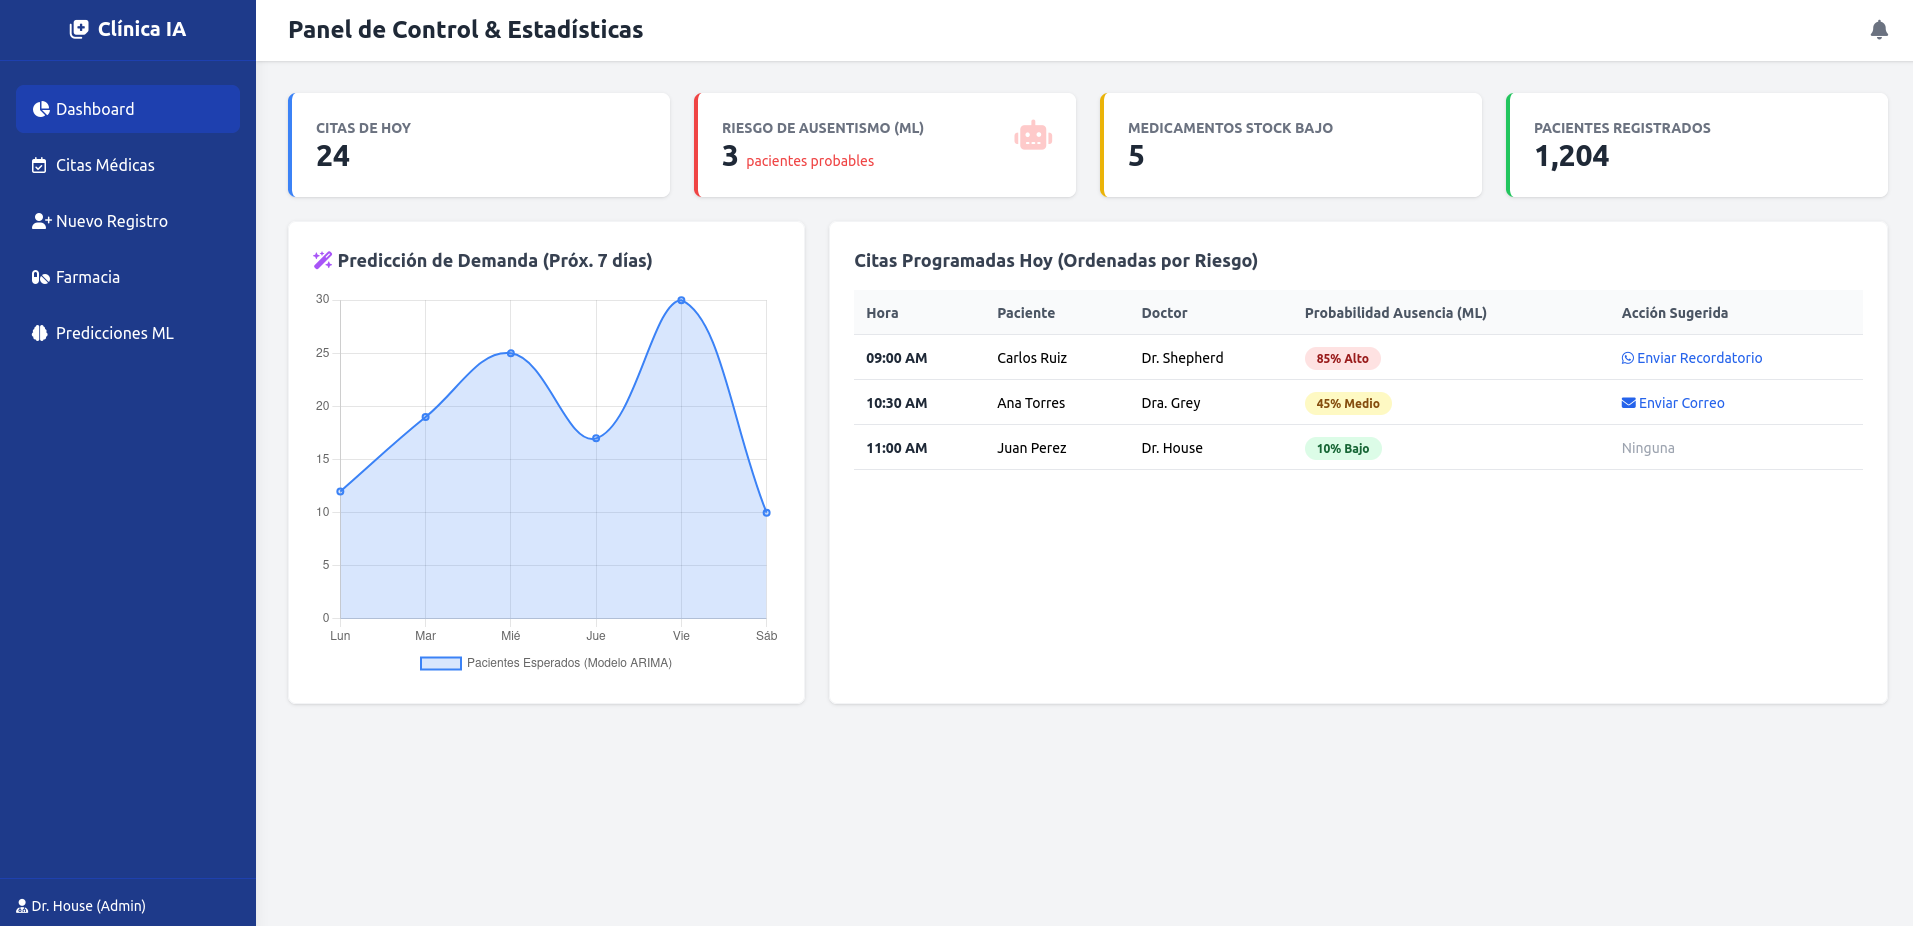
\includegraphics[width=0.7\textwidth]{dashboard.png}
	
		\caption{Panel Inicial con datos Estadisticos}
	\end{figure}
	
	\subsection{Interfaz de registro de citas}
	\begin{figure}[H]
		\centering
		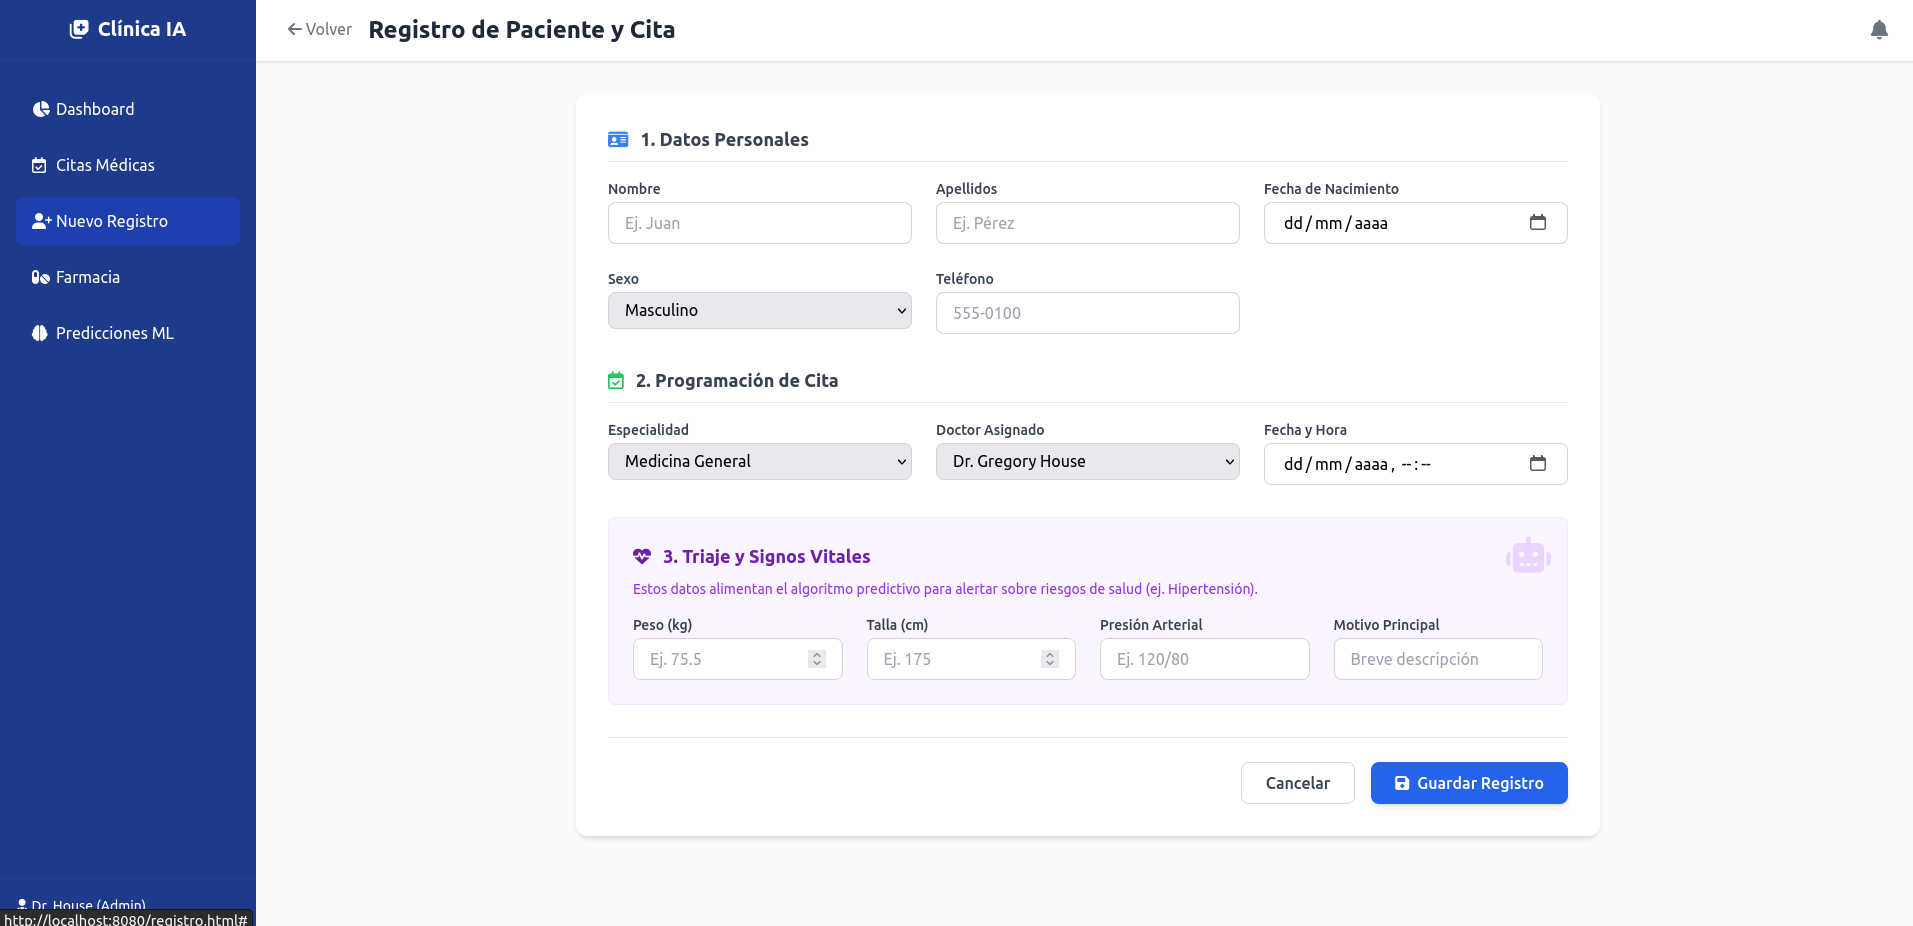
\includegraphics[width=0.7\textwidth]{registro.png}
		
		\caption{Registro de citas y asignaciones}
	\end{figure}
	
\end{document}

```